\documentclass{standalone}
\usepackage{tikz}

\usetikzlibrary{calc,shadows}


\begin{document}

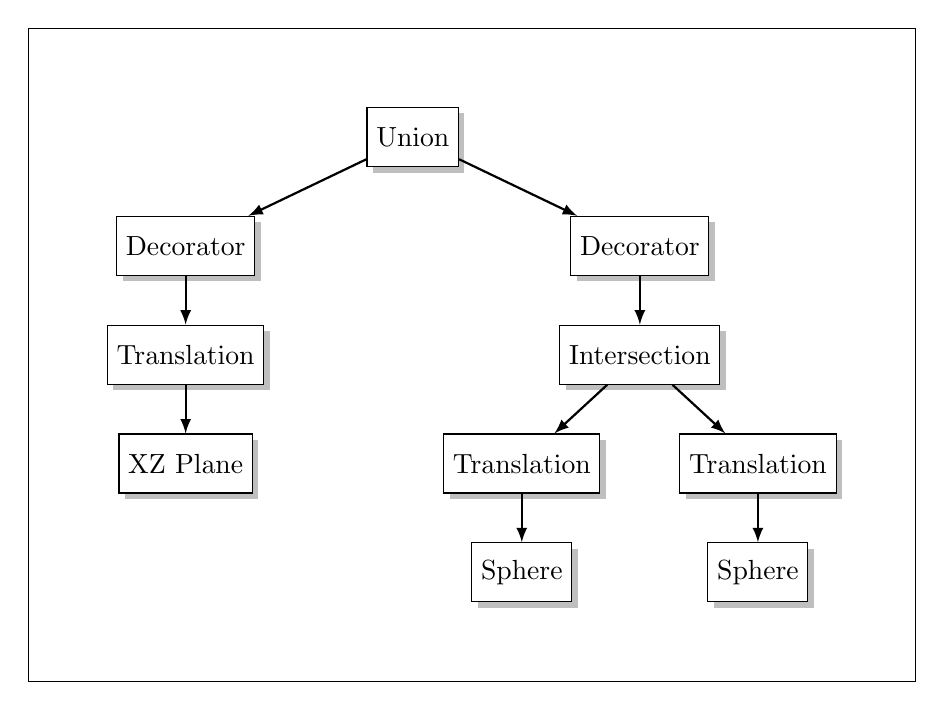
\begin{tikzpicture}[object/.style={draw,minimum height=.75cm,fill=white,drop shadow},link/.style={thick}, arrow/.style={-latex,thick}]
  \node[object] (root) {Union};
  \node[object,anchor=north east] (floor decorator) at ($ (root) + (-2,-1) $) {Decorator};
  \node[object,anchor=north] (floor translation) at ($ (floor decorator) + (0,-1) $) {Translation};
  \node[object,anchor=north] (floor) at ($ (floor translation) + (0,-1) $) {XZ Plane};
  \node[object,anchor=north west] (lens decorator) at ($ (root) + (2,-1) $) {Decorator};
  \node[object,anchor=north] (lens intersection) at ($ (lens decorator) + (0,-1) $) {Intersection};
  \node[object,anchor=north east] (translation1) at ($ (lens intersection) + (-0.5,-1) $) {Translation};
  \node[object,anchor=north west] (translation2) at ($ (lens intersection) + (0.5,-1) $) {Translation};
  \node[object,anchor=north] (sphere1) at ($ (translation1) + (0,-1) $) {Sphere};
  \node[object,anchor=north] (sphere2) at ($ (translation2) + (0,-1) $) {Sphere};

  \draw[arrow] (root) -- (floor decorator);
  \draw[arrow] (floor decorator) -- (floor translation);
  \draw[arrow] (floor translation) -- (floor);
  \draw[arrow] (root) -- (lens decorator);
  \draw[arrow] (lens decorator) -- (lens intersection);
  \draw[arrow] (lens intersection) -- (translation1);
  \draw[arrow] (lens intersection) -- (translation2);
  \draw[arrow] (translation1) -- (sphere1);
  \draw[arrow] (translation2) -- (sphere2);

  \draw let \p1=(sphere1.south), \p2=(translation2.east), \p3=(floor translation.west), \p4=(root.north) in
        ($ (\x3, \y1) + (-1,-1) $) rectangle ($ (\x2,\y4) + (1,1) $);
\end{tikzpicture}

\end{document}